\subsection*{\underline{تغییرات نمودار در راستای انطباق بر SQL و نرمال‌تر سازی}}

\textbf{در تمامی عکس‌های این بخش، عکس سمت راست معادل پیش از تغییرات است و عکس سمت چپ معادل پس از تغییرات است. دلیل برخی از تغییرات در ادامه به دلیل تکراری بودن ذکر نشده است.
}

$\\$

\includegraphics[width=0.5\linewidth]{figs/1-1.png} \
\includegraphics[width=0.5\linewidth]{figs/1-2.png}

اگریگیشن  در SQL وجود ندارد. بنابراین باید شکسته شود. در اینجا تصمیم بر این شد که کاربر و حساب کاربری به دلیل داشن رابطه 1:1 و ویژگی‎های تقریباً مرتبط تبدیل به یک موجودیت شوند و تمام روابطی که به این اگریگیشن متصل است، به userAccount وصل شود.

$\\$

\includegraphics[width=0.5\linewidth]{figs/2-1.jpg} \
\includegraphics[width=0.5\linewidth]{figs/2-2.jpg}

در گام بعد باید همه روابط manyToMany شکسته شوند. در اینجا رابطه بین discountCode و userAccount باید شکسته شود. برای این کار این رابطه را به دو رابطه تبدیل میکنیم که یکی از آنها مربوط به دریافت‎کننده و دیگری مربوط به اهداکننده کد تخفیف است.

\pagebreak

\includegraphics[width=0.5\linewidth]{figs/3-1.jpg} \
\includegraphics[width=0.5\linewidth]{figs/3-2.jpg}

در اینجا بین trip و terminal رابطه m:n برقرار بود زیرا از هر ترمینال چند سفر انجام می‎شود و هر سفر یک ترمینال مبدا و یک ترمینال مقصد دارد. حالا باید این رابطه را تبدیل به دو رابطه اکنیم که یکی مبدا را مشخص می‎کند و یکی مقصد را.


\includegraphics[width=0.5\linewidth]{figs/4-1.jpg} \
\includegraphics[width=0.5\linewidth]{figs/4-2.jpg}

رابطه بین reservation و discountCode هم m:n بود چون هر کد تخفیف ممکن است بر چند رزرو اعمال شود و هر رزرو چند کد تخفیف داشته باشد. برای حل مشکل می‎توانیم یک موجودیت  ضعیف discountUsage داشته باشیم که کلید خارجی به این دو موجودیت داشته باشد و مشخص کند هر استفاده‎ای از کد تخفیف مربوط به چه کد تخفیفی و برای چه رزروی است.

$\\$

\includegraphics[width=0.5\linewidth]{figs/5-1.jpg} \
\includegraphics[width=0.5\linewidth]{figs/5-2.jpg}

مورد دیگری که در SQL وجود ندارد ولی در نمودار ما بود، specialization است. برای حل این مشکل موجودیت کلی‎تر را حذف می‎کنیم، و تمام attributeها و روابط آن را به همه موجودیت‎های جزئی آن نسبت می‎دهیم.

$\\$

\includegraphics[width=0.5\linewidth]{figs/6-1.jpg} \
\includegraphics[width=0.5\linewidth]{figs/6-2.jpg}



$\\$

\includegraphics[width=0.5\linewidth]{figs/7-1.jpg} \
\includegraphics[width=0.5\linewidth]{figs/7-2.jpg} 



$\\$
\includegraphics[width=0.5\linewidth]{figs/8-1.jpg} \
\includegraphics[width=0.5\linewidth]{figs/8-2.jpg} 




$\\$
\includegraphics[width=0.5\linewidth]{figs/9-1.jpg} \
\includegraphics[width=0.5\linewidth]{figs/9-2.jpg} 




$\\ \\$
\includegraphics[width=0.5\linewidth]{figs/10-1.jpg} \
\includegraphics[width=0.5\linewidth]{figs/10-2.jpg} 



$\\$
\includegraphics[width=0.5\linewidth]{figs/11-1.jpg} \
\includegraphics[width=0.5\linewidth]{figs/11-2.jpg} 





$\\$
\includegraphics[width=0.5\linewidth]{figs/12-1.jpg} \
\includegraphics[width=0.5\linewidth]{figs/12-2.jpg} 



$\\$
\includegraphics[width=0.5\linewidth]{figs/13-1.jpg} \
\includegraphics[width=0.5\linewidth]{figs/13-2.jpg} 


$\\$
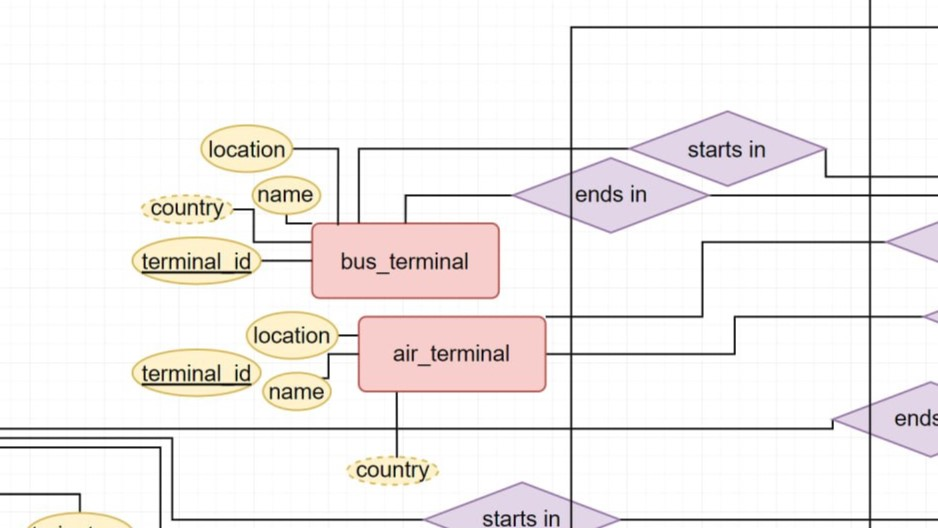
\includegraphics[width=0.5\linewidth]{figs/14-1.jpg} \


در همه انواع ترمینال لوکیشن میتواند کشور را مشخص کند، و لوکیشن یک ck نیست. برای تبدیل به 3nf باید این مورد رفع شود. یک موجودیت ضعیف برای این مورد میسازیم و ویژگی کشور را از ترمینال حذف میکنیم.

$\\$
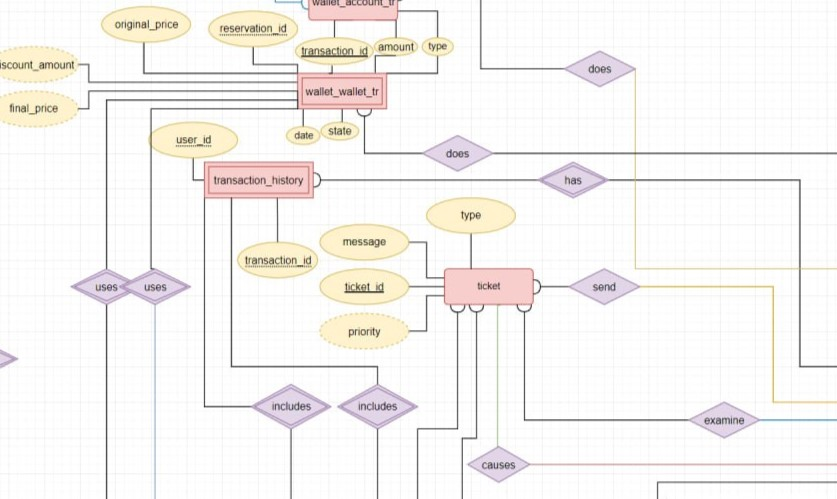
\includegraphics[width=0.5\linewidth]{figs/15-1.jpg} \


در اینجا هم بین type و priority وابستگی وجود دارد. به همین دلیل این دو را در جدولی جدا درج کردیم که اصول 3nf برقرار باشد.



$\\$
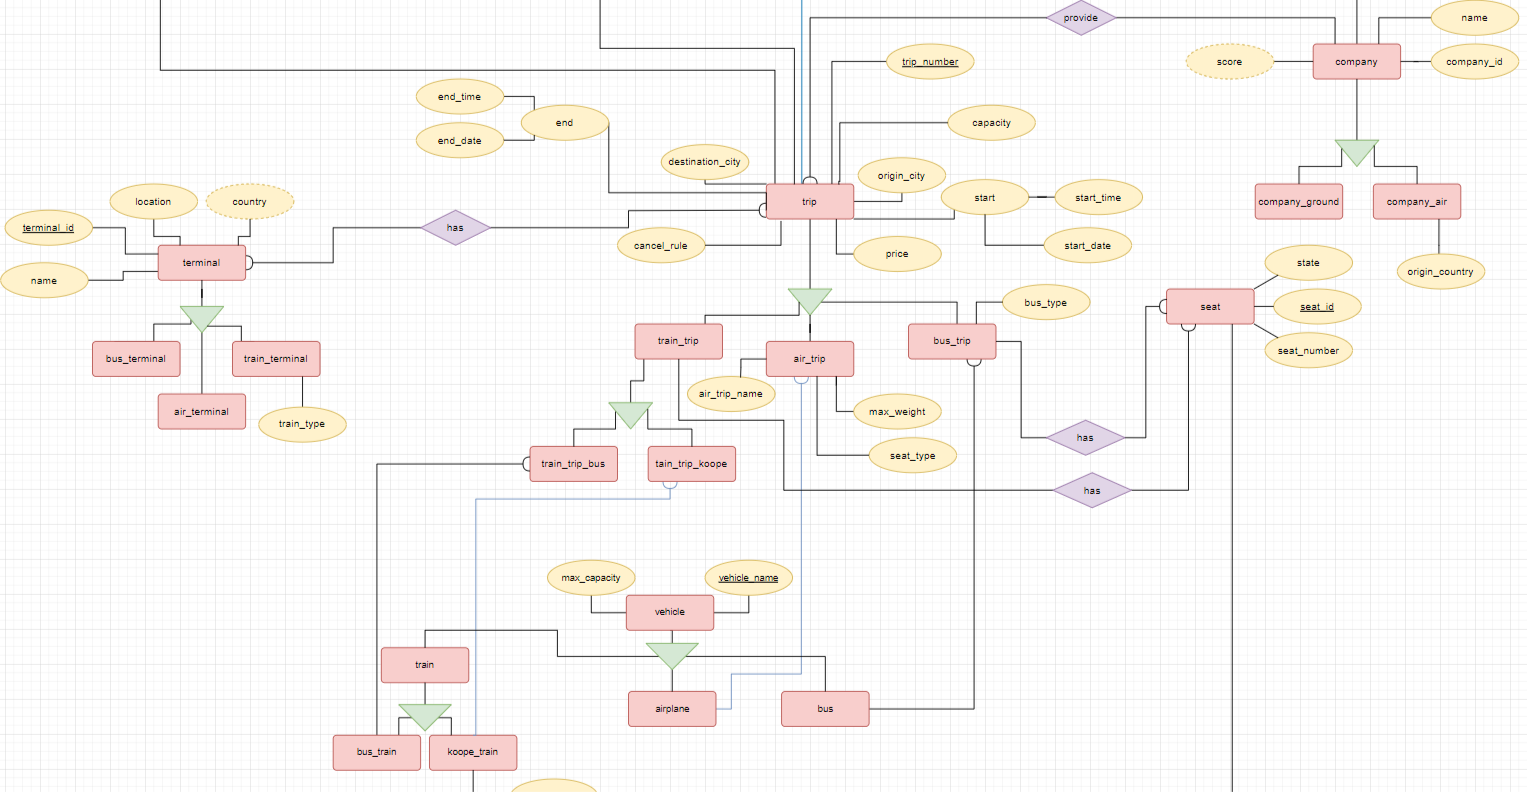
\includegraphics[width=0.5\linewidth]{figs/16-1.png} \
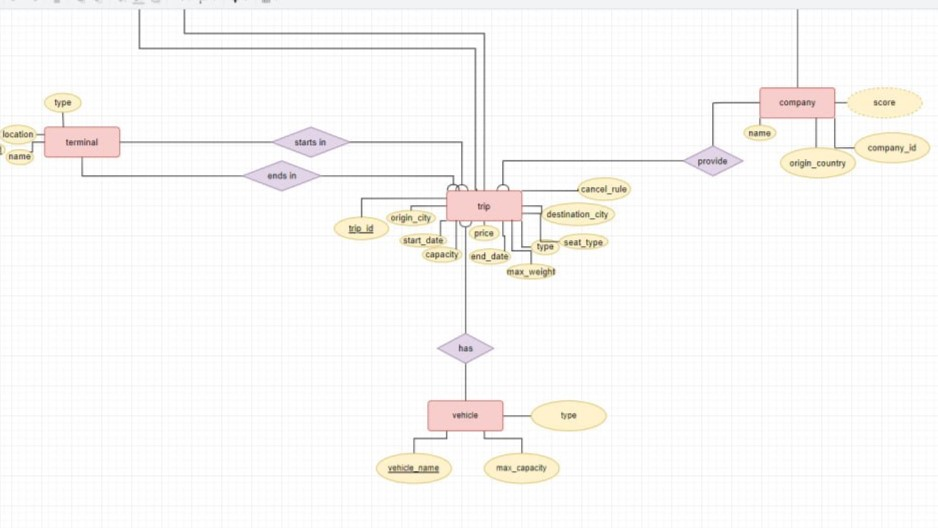
\includegraphics[width=0.5\linewidth]{figs/16-2.jpg} 


در حین پیاده‌سازی جداول متوجه شدیم که بسیاری از موجودیت‌هایی که به صورت انواع مختلفی از یک موجودیت جدا کردیم (specialization)، میتوانند همگی یک موجودیت باشند که نوعشان در اتریبیوتی به نام type ذخیره شود:

$\\$
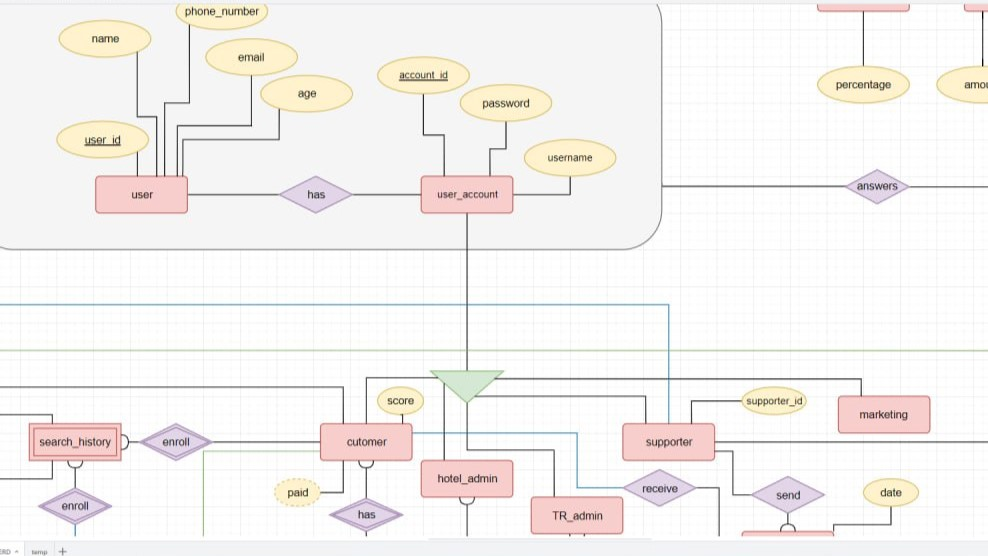
\includegraphics[width=0.5\linewidth]{figs/17-1.jpg} \
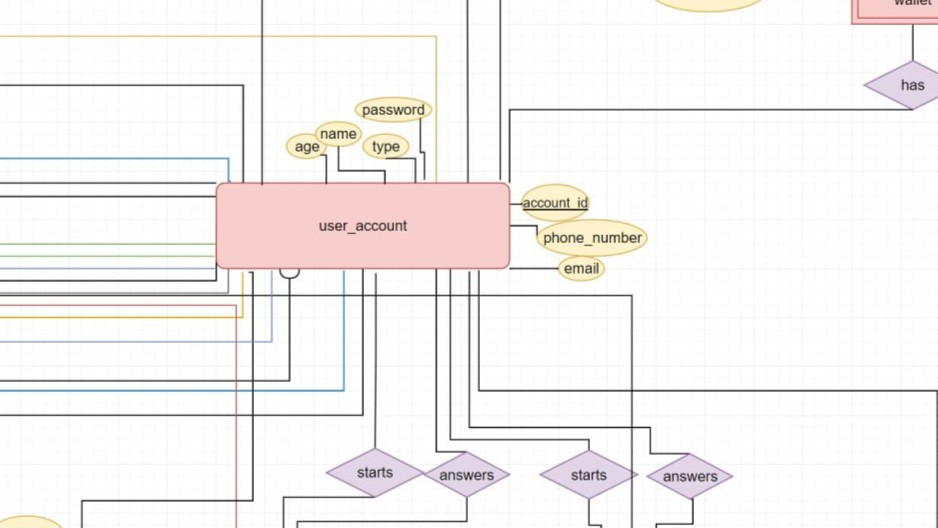
\includegraphics[width=0.5\linewidth]{figs/17-2.jpg} 

همچنین دریافتیم که نیاز است برخی از موجدیت‌ها به دو موجودیت جداگانه شکسته شوند. دلیل این موضوع، foreign keyهایی بود که مشخص نبود باید دقیقاً به کدام موجودیت اشاره کنند (دو حالت داشتند).

$\\$
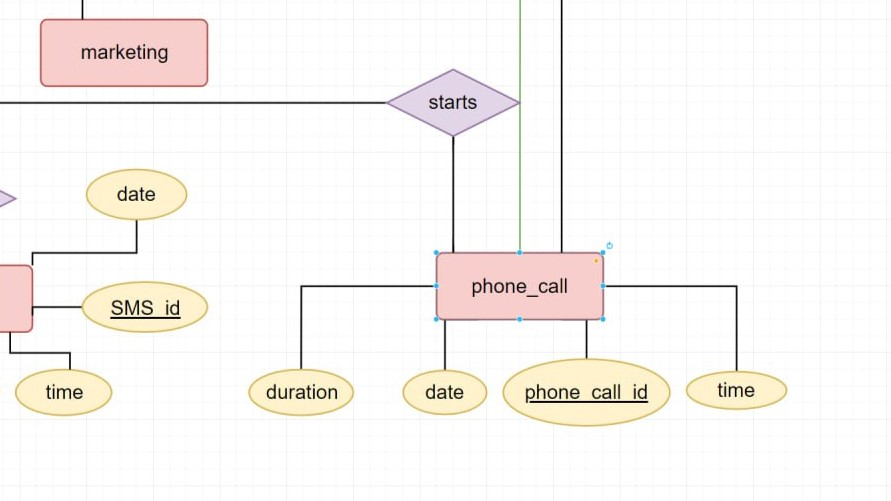
\includegraphics[width=0.5\linewidth]{figs/18-1.jpg} \
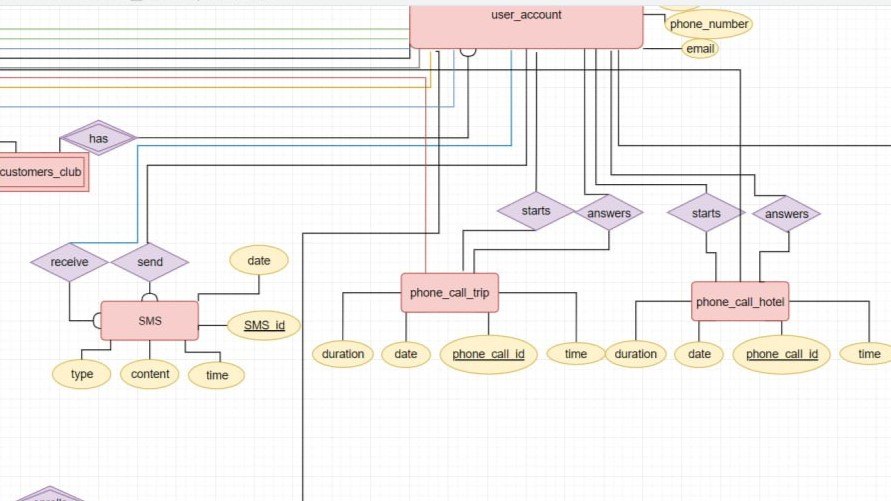
\includegraphics[width=0.5\linewidth]{figs/18-2.jpg} 

$\\$
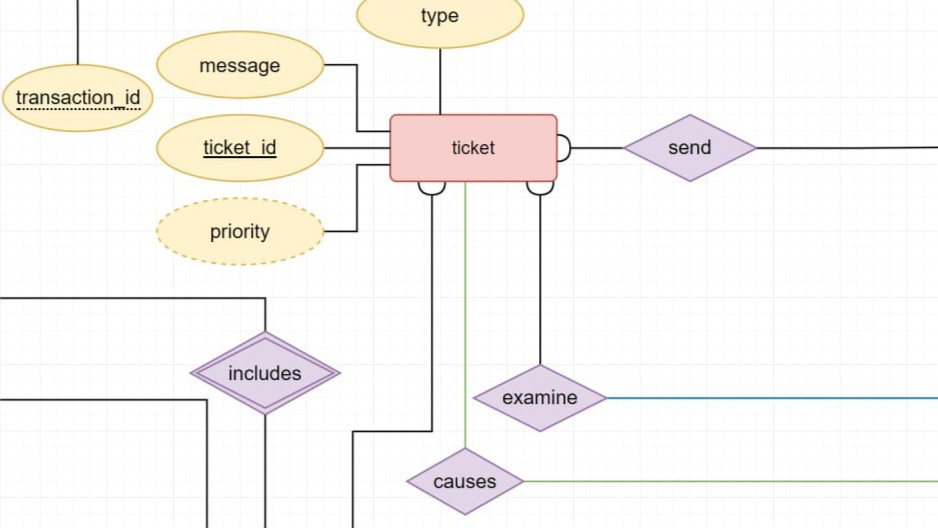
\includegraphics[width=0.5\linewidth]{figs/19-1.jpg} \
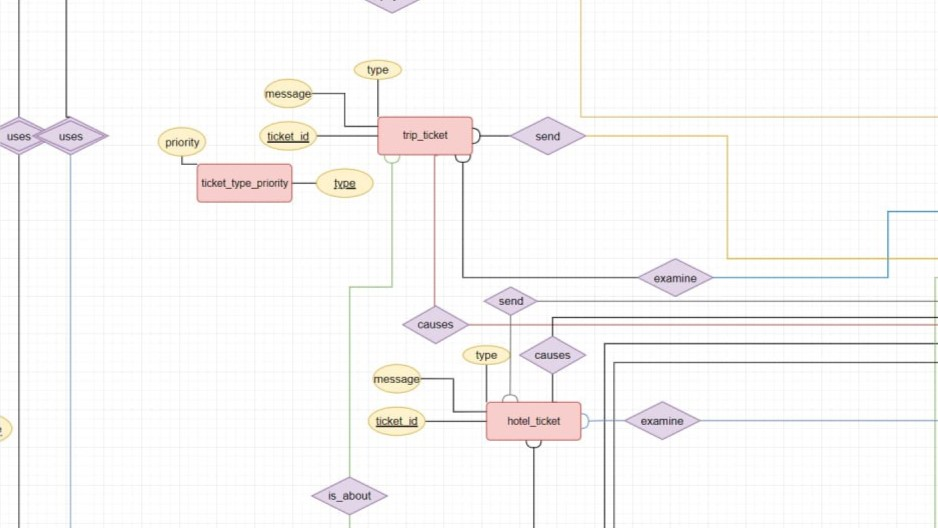
\includegraphics[width=0.5\linewidth]{figs/19-2.jpg} 

\pagebreak

در همه انواع ترمینال لوکیشن میتواند کشور را مشخص کند، و لوکیشن یک ck نیست. برای تبدیل به 3nf باید این مورد رفع شود. یک موجودیت ضعیف برای این مورد میسازیم و ویژگی کشور را از ترمینال حذف میکنیم.

\setLTR
pageterminal-id — < location

location — < country
\setRTL


این یک transitive dependency است.
(در اینجا فرض شده که ممکن است دو ترمینال لوکیشن‎های مشابه داشته باشند.)


$\\$
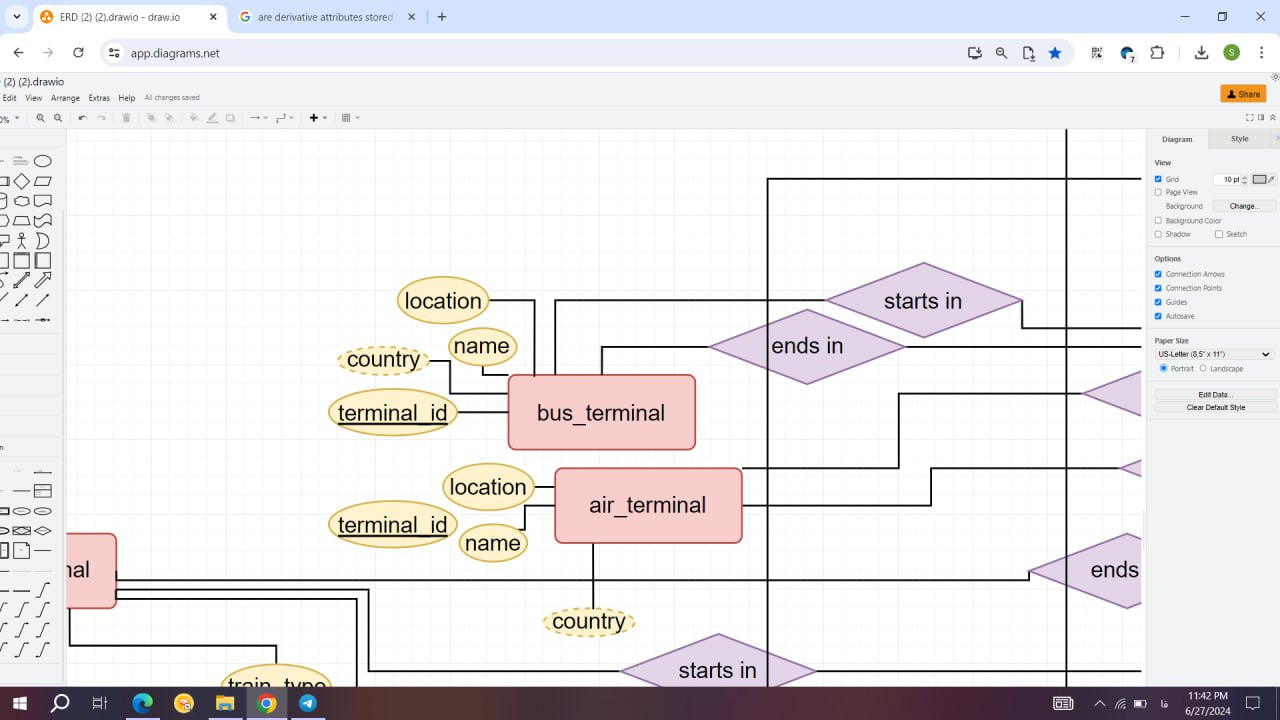
\includegraphics[width=0.7\linewidth]{figs/a1.jpg} \


در اینجا هم بین type و priority وابستگی وجود دارد.

\setLTR
ticket-id — < type

type — < priority
\setRTL

این یک transitive dependency است که با 3nf در تناقض است. بنابراین باید priority از این تیبل خارج شود و در جدولی قرار داده شود که تایپ، primary key آن است.

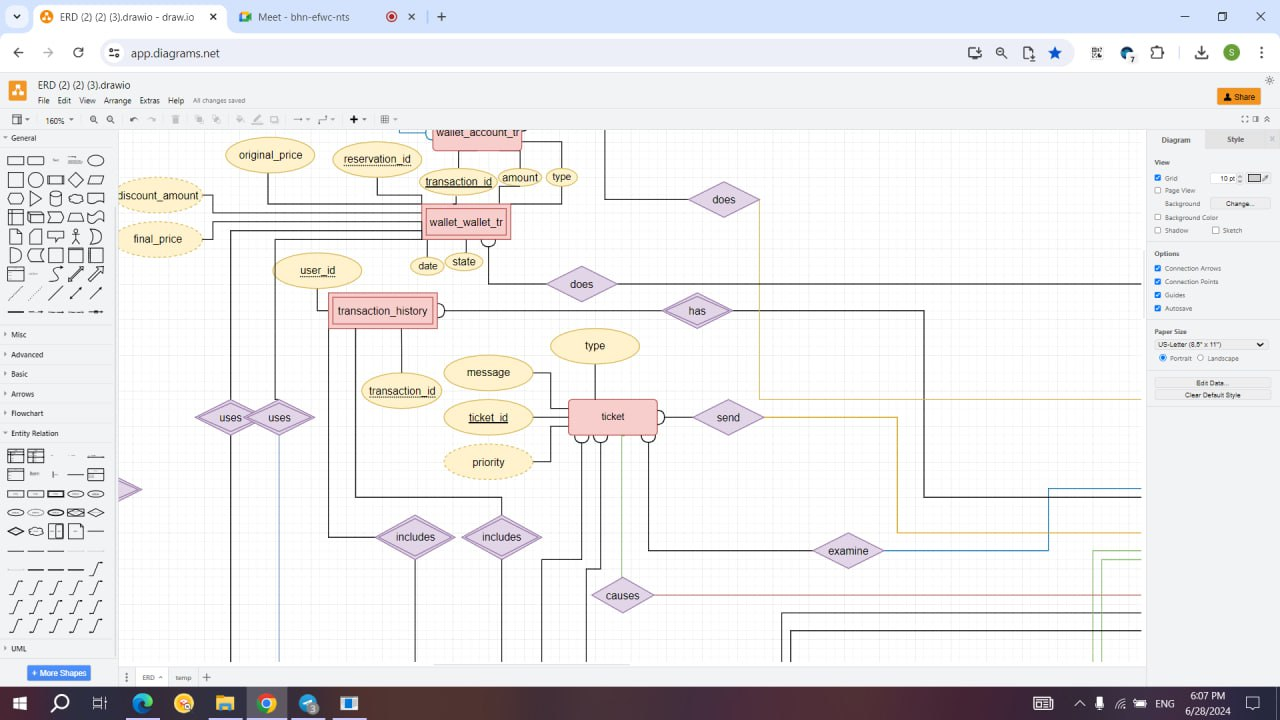
\includegraphics[width=0.7\linewidth]{figs/a2.jpg} \

\pagebreak

$\\ \\$
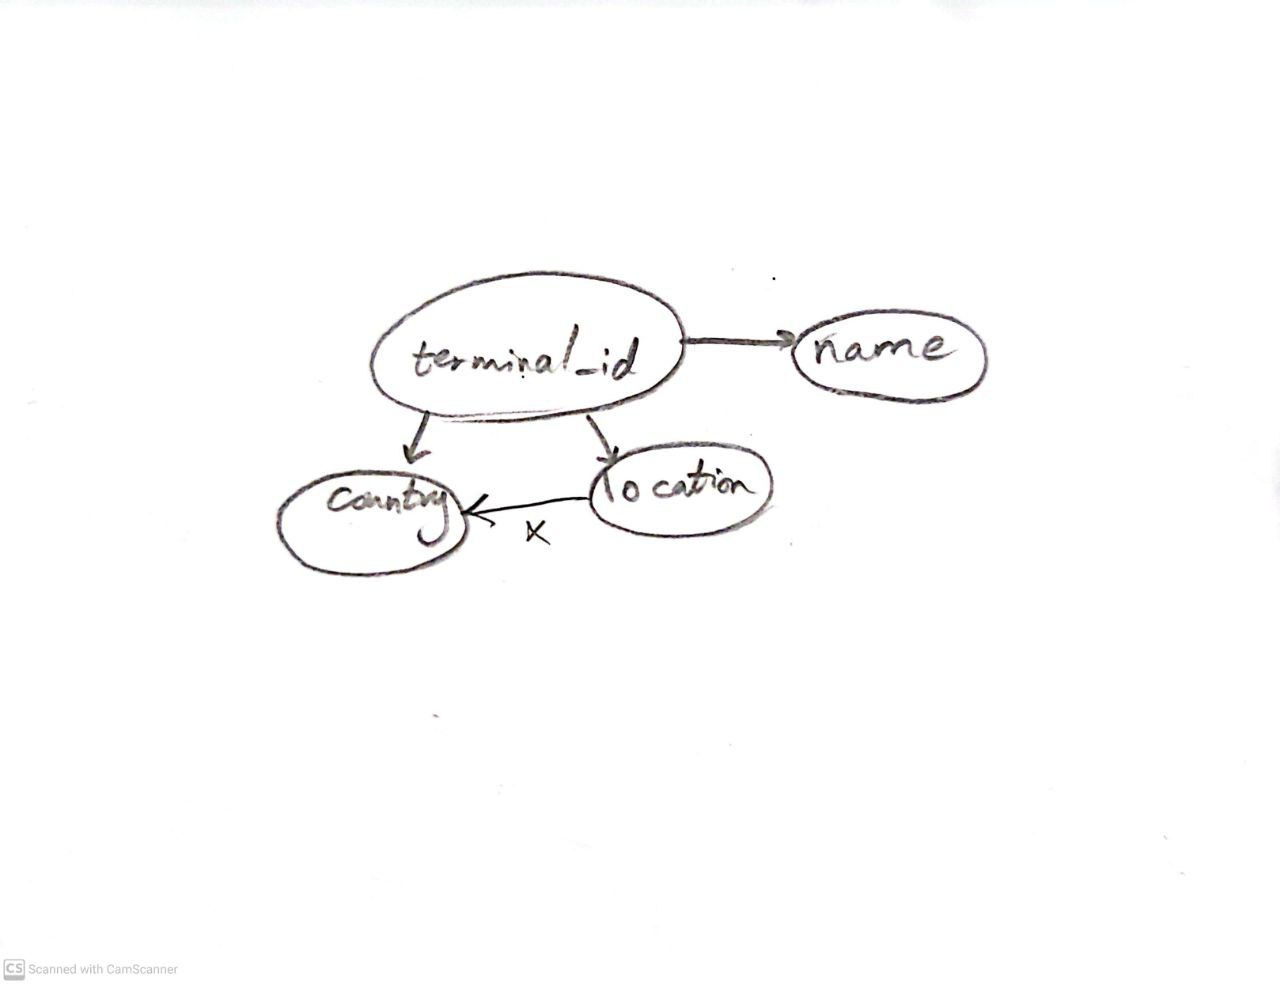
\includegraphics[width=0.7\linewidth]{figs/b1.jpg} \
$\\$
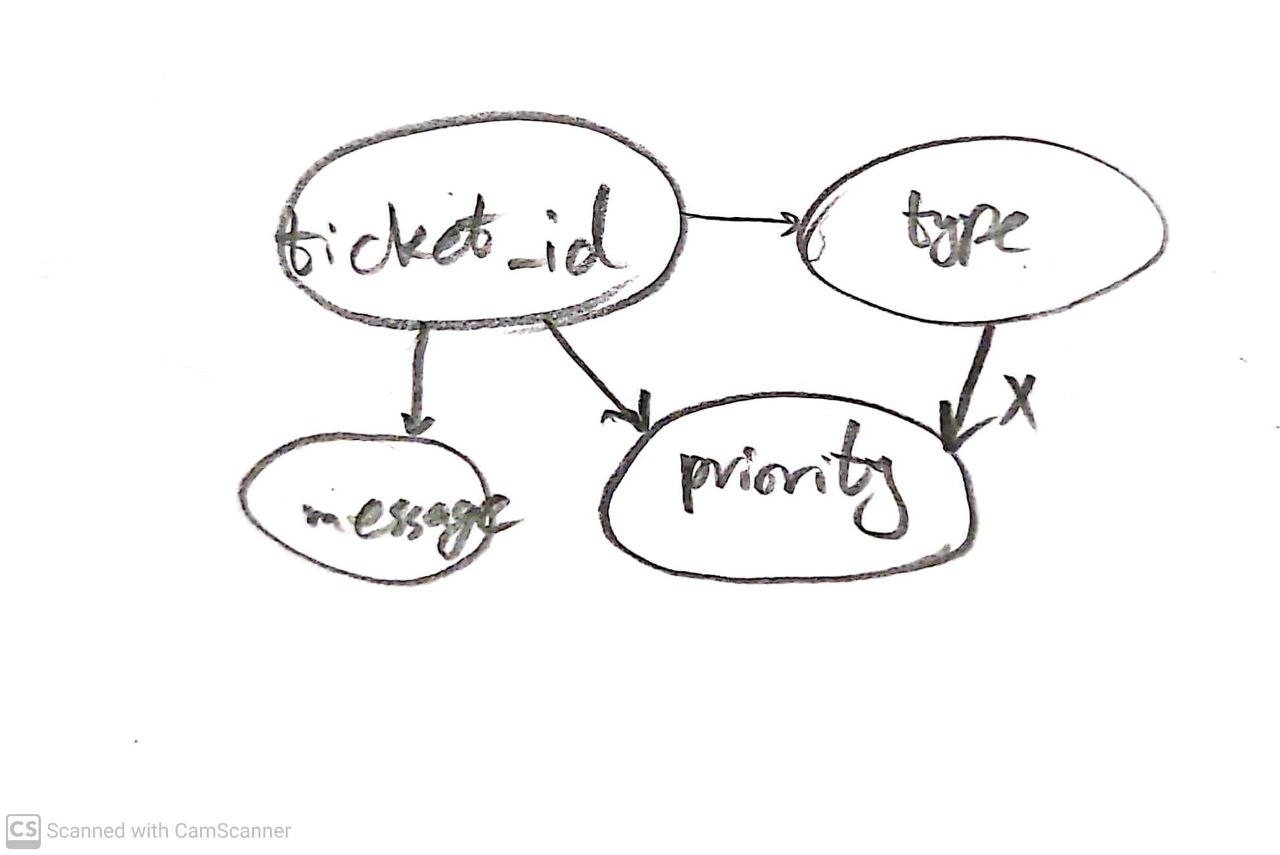
\includegraphics[width=0.7\linewidth]{figs/b2.jpg} \